\documentclass{beamer}
%\usetheme{default}
%\usetheme{AnnArbor}
%\usetheme{Antibes}
%\usetheme{Bergen}
%\usetheme{Berkeley}
%\usetheme{Berlin}
%\usetheme{Boadilla}
%\usetheme{CambridgeUS}
%\usetheme{Copenhagen}
%\usetheme{Darmstadt}
%\usetheme{Dresden}
%\usetheme{Frankfurt}
%\usetheme{Goettingen}
%\usetheme{Hannover}
%\usetheme{Ilmenau}
%\usetheme{JuanLesPins}
%\usetheme{Luebeck}
\usetheme{Madrid}
%\usetheme{Malmoe}
%\usetheme{Marburg}
%\usetheme{Montpellier}
%\usetheme{PaloAlto}
%\usetheme{Pittsburgh}
%\usetheme{Rochester}
%\usetheme{Singapore}
%\usetheme{Szeged}
%\usetheme{Warsaw}
\setbeamertemplate{navigation symbols}{}

%\usecolortheme{albatross}
\usecolortheme{beaver}
%\usecolortheme{beetle}
%\usecolortheme{crane}
%\usecolortheme{dolphin}
%\usecolortheme{dove}
%\usecolortheme{fly}
%\usecolortheme{lily}
%\usecolortheme{orchid}
%\usecolortheme{rose}
%\usecolortheme{seagull}
%\usecolortheme{seahorse}
%\usecolortheme{whale}
%\usecolortheme{wolverine}

\usepackage{tikz}
\usepackage{graphicx}
\graphicspath{{../Images/}}
\usepackage{multicol}
\usepackage{ulem}
\normalem

\usepackage{amsmath}
\DeclareMathOperator*{\argmax}{arg\,max}



\title[Stat 185 - Overview]{Statistics 185 - Introduction to Dimension Reduction}
\subtitle{Course Introduction and Overview}
\author{Instructor: Alex Young} 
\date{Tuesday September 3}


\begin{document}

\begin{frame}
\titlepage
\end{frame}

\section{What is high-dimensional data?}
\begin{frame}{Examples of High-Dimensional data}
\begin{block}{Ubiquitous in the modern data-driven economy}
\begin{itemize}
\item Static Images
\begin{itemize}
	\item Handwritten digits, signature
	\item Medical images
\end{itemize}
\item Movies/Audio/Signals
\item Genetic data
	\begin{itemize}
		\item Personalized medicine
		\item Genotype/phenotype connections
	\end{itemize}
\item Textual data
\begin{itemize}
	\item Spam detection
\end{itemize}
\item Patient and consumer data
\begin{itemize}
	\item Who is likely to buy (or die)?
\end{itemize}
\end{itemize}
\end{block}

\end{frame}

\begin{frame}{What is high-dimensional?}
\begin{block}{Depends on the number of samples?}
Consider the $d$-dimensional box $[0,1]^d$ divided into bins by cutting 10 slabs in each direction.
\begin{multicols}{2}

\begin{figure}
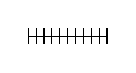
\begin{tikzpicture}
\draw[step= 0.1] (0,0) -- (1,0);
\foreach \i in {0, ..., 10}{
\draw (\i/10, -0.1) -- (\i/10, 0.1);
}
\end{tikzpicture}
\caption{1D $\rightarrow$ 10 bins}
\end{figure}

\begin{figure}
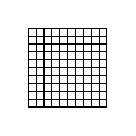
\begin{tikzpicture}
\draw[step = 0.1] (0,0) grid (1,1); 
\end{tikzpicture}
\caption{2D $\rightarrow$ 100 bins}
\end{figure}


\end{multicols}
\end{block}\pause

\begin{block}{Exponential in the number of samples}
\begin{itemize}
\item If we want to make one observation in each bin, we need $10^d$ samples. 
\item A $19 \times 19$ pixel image translates to {\bf one}  $19^2$-dimensional datum.
\begin{itemize}
	\item Need $10^{381}$ samples
	\item Estimated $10^{82}$ atoms in the universe!
\end{itemize}
\item Assumes uniform distribution but the idea generalizes.
\end{itemize}
 

\end{block}

\end{frame}


\section{What is Dimension Reduction?}

\begin{frame}{One name, many goals}

\begin{block}{Curse of Dimensionality (Bellman)}
\begin{itemize}
\item High dimension $\rightarrow$ sparse data
	\begin{itemize}
	\item Need exponentially increasing (in dimension samples), otherwise ... \pause 
	\item Model + High-dimensional data  $=$ Overfitting (often) \pause
	\end{itemize}
\item Model + Reduced dimensions  = Generalizability (hopefully) \pause
\end{itemize}

\end{block}

\begin{block}{Reasons for Dimension Reduction}
\begin{itemize}
\item Feature extraction or selection \pause
\item Learn geometric features from data that cannot be visualized \pause
\item Data compression \pause
\item Reduced computation cost  \pause
\item Removal of redundant information
\end{itemize}
\end{block}
\end{frame}


\begin{frame}{Example - Nonnegative Matrix Factorization}
\begin{center}
\begin{figure}[h!]
\includegraphics[width = 0.9\textwidth]{Hastie-Faces-NMF}
\caption{Image taken from \emph{Elements of Statistical Learning} by Hastie, Tibshirani, and Friedman, originally from Lee and Seung (1999)}
\end{figure}
\end{center}
\end{frame}

\begin{frame}{Example - Vector Quantization/$k$-means}
\begin{center}
\begin{figure}[h!]
\includegraphics[width = 0.9\textwidth]{Hastie-Faces-VQ}
\caption{Image taken from \emph{Elements of Statistical Learning} by Hastie, Tibshirani, and Friedman, originally from Lee and Seung (1999)}
\end{figure}
\end{center}
\end{frame}


\begin{frame}{Example - Principal Component Analysis}
\begin{center}
\begin{figure}[h!]
\includegraphics[width = 0.9\textwidth]{Hastie-Faces-PCA}
\caption{Image taken from \emph{Elements of Statistical Learning} by Hastie, Tibshirani, and Friedman, originally from Lee and Seung (1999)}
\end{figure}
\end{center}
\end{frame}

\begin{frame}{Example - Principal Component Analysis}
\begin{center}
\begin{figure}
\includegraphics[width = 0.5 \textwidth]{Hastie-Digitized_Threes}
\includegraphics[width = 0.7\textwidth]{Hastie-Three-PCA}
\caption{Images and equation taken from \emph{Elements of Statistical Learning} by Hastie, Tibshirani, and Friedman}
\end{figure}
\end{center}
\end{frame}

\begin{frame}{Hierarchical Clustering}
\begin{center}
\begin{figure}
\includegraphics[width = 0.9 \textwidth]{Izenman-Hierarchical_Clustering}
\caption{Image taken from \emph{Modern Multivariate Statistical Techniques} by Izenman}
\end{figure}
\end{center}
\end{frame}

\begin{frame}{Hierarchical Clustering}
\begin{center}
\begin{figure}
\includegraphics[height = 0.7 \textheight]{Hastie-Hierarchical_Clustering}
\caption{Image of Hierarchical Clustering for tumor microarray data taken from \emph{Elements of Statistical Learning} by Hastie, Tibshirani, and Friedman}
\end{figure}
\end{center}
\end{frame}

\begin{frame}{Spectral Clustering}
\begin{center}
\begin{figure}[h!]
\includegraphics[height = 0.7\textheight]{Hastie-Spectral_Clustering}
\caption{Image taken from \emph{Elements of Statistical Learning} by Hastie, Tibshirani, and Friedman}
\end{figure}
\end{center}
\end{frame}



\begin{frame}{Taxonomy of Dimension Reduction (by Convexity) }
\begin{center}
\begin{figure}[h!]
\includegraphics[height = 0.75\textheight]{Taxonomy_of_DR_by_Convexity}
\end{figure}
\end{center}
\footnotesize{Image from \emph{dimRed and coRanking—Unifying Dimensionality Reduction in R} by
Guido Kraemer, Markus Reichstein, and Miguel D. Mahecha}
\end{frame}


\begin{frame}{Taxonomy of Dimension Reduction (by Linearity) }
\begin{center}
\begin{figure}[h!]
\includegraphics[height = 0.75\textheight]{Taxonomy_of_DR_by_Linearity}
\end{figure}
\end{center}
\footnotesize{Image from \emph{Dimensionality Reduction: A Comparative Review} by Laurens van der Maaten, 
Eric Postmam, and
H. Jaap Van Den Herik
}
\end{frame}


\section{Course Description}
\begin{frame}{Course Objectives}


\begin{block}{Recent trends in Dimension Reduction Research}
\begin{itemize}
\item Google Scholar results for `Dimension Reduction' search
\begin{itemize}
\item 2017 - 88,000 articles
\item 2018 - 72,700 articles
\item 2019 - 40,000 articles
\end{itemize}
\item Expanded into more specialized subfields, i.e. manifold learning \pause
\end{itemize}
\end{block}
\begin{block}{An Enormous and Active Field}
\begin{itemize}
\item Many missing topics from previous slides
\begin{itemize}
\item Specialized (variants of existing) algorithms being developed for specific needs
\item Primary focus of listed techniques is on continuous data
\item Graphical and/or discrete data receiving increased interest
\end{itemize}

\item Implementation for massive datasets drives parallel research in computation
\begin{itemize}
\item Messy landscape of competing codes, packages, and applications
\end{itemize}
\end{itemize}
\end{block}
\end{frame}

\begin{frame}{Course Objectives}
\begin{block}{An introduction to the field}
\begin{itemize}
\item Cannot give an exhaustive summary
\begin{itemize}
\item Field is still evolving $\rightarrow$ ever-expanding list of topics
\item Best computational tool(s) is a topic of much debate
	\begin{itemize}
	\item Computation alone can miss important insight
	\end{itemize}
\end{itemize}
\item High-dimensional geometry can be \sout{challenging} \sout{counterintuitive} weird
\begin{itemize}
\item Cannot directly visualize to detect patterns in data
\item Different techniques $\rightarrow$ different behaviors/goals $\rightarrow$ different insights
	\begin{itemize}
	 \item Manifold Learning, Clustering/Grouping, Classification, etc \pause
	\end{itemize}
\end{itemize}
\end{itemize}
\end{block}
\begin{block}{Goal: Learn to critique}
\begin{itemize}
\item Demonstrate the practice of using careful analysis to explore (classic) techniques with the aim of learning:
\begin{itemize}
\item What behavior(s) they aim to capture
\item Their strengths, weaknesses, limitations, and challenges 
\item When they will work and when they are likely to fail
\end{itemize}
\end{itemize}
\end{block}
\end{frame}


\begin{frame}{Commonalities across Methods}
\begin{block}{Data $\rightarrow$ Vectors}
\begin{itemize}
\item Observe $d$ variables from $N$ subjects, i.e. $N$ vectors in $\mathbb{R}^d$
\item Mean $\rightarrow$ vector; Covariance $\rightarrow$ Matrix
	\begin{itemize}
		\item \emph{Multivariate probability/statistics} \pause
	\end{itemize}
\end{itemize}
\end{block}

\begin{block}{What does the cloud of data points look like?}
\begin{itemize}
	\item If we could view the points, are they concentrated on/near some shape of lower dimension?
		\begin{itemize}
			\item e.g. Observations in $\mathbb{R}^3$ near a smooth curve/line
			\item e.g. Observations in $\mathbb{R}^{381}$ near a $71$-dimensional affine subspace?
		\end{itemize}
	\item If we cannot visualize, how can we make sense of the geometric features?
		\begin{itemize}
			\item \emph{Linear algebra}
		\end{itemize}
\end{itemize}
\end{block}

\end{frame}

\begin{frame}{Commonalities across Methods}
\begin{block}{Central Assumption}
\begin{itemize}
	\item There is some lower dimensional structure inherent to the data! \pause
\end{itemize}
\end{block}

\begin{block}{Goal: Minimal `information' loss}
\begin{itemize}
 \item Replace observation in $\mathbb{R}^d$ with compressed representation in $\mathbb{R}^k$ where $k \ll d$ 
 \item Different notions of `information', but maximization/minimization is common aim
 	\begin{itemize}
 		\item \emph{Optimization, Multivariable Calculus}
 	\end{itemize}
 	$$w^* = \argmax_{\| w\| = 1} \| X w\| $$
 	$$ (W^*,H^*) = \argmax \sum \sum [x_{ij} \log (WH)_{ij} - (WH)_{ij} ]$$
\end{itemize}
\end{block}

\end{frame}



\begin{frame}{Course Overview}
\begin{block}{Tentative Schedule}
{\small The proposed schedule could changed depending upon a myriad of factors. }
{\tiny 
\begin{center}
\renewcommand{\arraystretch}{1.25}
\begin{table}[h!]
\begin{tabular}{|c|c|c|c|c|}
\hline
Week & Date & Topic & Date & Topic \\
\hline
1 & 9/3&   Course Overview (HW\#1 out)  & 9/5 & Review: Multivar. Stats. \\
\hline
2 & 9/10 & 	 PCA	I (HW\#1 due) & 9/12& PCA II \\
\hline
3 & 9/17 & PCA III  (HW\#2 out)& 9/19 & CCA I    \\
 \hline 
 4 & 9/24 & CCA II  (HW\#2 due)& 9/26 & NMF I (HW\#3 out)   \\
 \hline
 5 & 10/1 &  NMF II   & 10/3 & NMF III (HW\#3 due)   \\
 \hline 
 6 & 10/8 & MDS I (HW\#4 out)  & 10/10 & MDS II \\
 \hline 
 7 & 10/15 & MDS III (HW\#4 due)   & 10/17 & Midterm (MT coding out)  \\ 
 \hline
 8 & 10/22 & ISOMAP  & 10/24 & LLE  (MT coding due)   \\ 
 \hline
 9 & 10/29 &  Probability Review(HW\#5 out) &10/31 &  Johnson-Lindenstrauss  \\
 \hline
 10 & 11/5 & Compressed Sensing (HW\#5 due)   & 11/7  &  Hierarchical Clustering (HW\#6 out)  \\
 \hline
 11 & 11/12 &  Center-based clustering  & 11/14 &  Spectral Clustering (HW\#6 due)    \\
 \hline
 12 & 11/19 &  Spectral Clustering (HW\#7 out) & 11/21 & Kernel Methods \\
 \hline
 13 & 11/26 &  Google PageRank (HW\#7 due)  & 11/28 & Thanksgiving: No class \\ 
 \hline
 14 & 12/3 &  Variational Autoencoder & 12/4 & Fall Reading Period: No class \\
 \hline
 Final Exam Period & 12/ & Term Papers Due &  & \\
\hline
\end{tabular}
\end{table}
\end{center}

}
\end{block}
\end{frame}

\begin{frame}{Course Layout - Assignments/Grading}
\begin{block}{Homework (40\%) }
\begin{itemize}
\item 7 total assignments, lowest score dropped
	\begin{itemize}
		\item Homework \#1 available on Canvas (due next Tuesday)
	\end{itemize}
\item Each assignment will include some (guided) coding portions in R
	\begin{itemize}
		\item \underline{Experience in R a plus but not required}
		\item Interface through RStudio
	\end{itemize}
\item RMarkdown files, complete and submit through Canvas as pdf/html
	\begin{itemize}
		\item \underline{Write answers in Markdown (similar to \LaTeX)}
		\item Good preparation for writing/formatting term paper (more on this shortly)
	\end{itemize}
\item Encouraged to work together, but must submit solutions written in your own words
\end{itemize}
\end{block}


\end{frame}


\begin{frame}{Course Layout - Assignments/Grading}
\begin{block}{Midterm (20\%)}
\begin{itemize}
\item Written portion (10\%)
	\begin{itemize}
		\item In-class on Thursday October 17th
		\item To cover PCA through MDS (see calendar)
		\item Similar content to homework sets
		\item Detailed discussion on layout/content of the exam on Tuesday October 15th
	\end{itemize}
\item Coding portion (10\%)
	\begin{itemize}
		\item Released Thursday October 17th; Due Thursday October 24th
		\item RMarkdown file similar to homework
		\item No collaboration allowed but Office Hours encouraged!
	\end{itemize}
\end{itemize}
\end{block}

\end{frame}


\begin{frame}{Course Layout - Assignments/Grading}
\begin{block}{Term Paper (40\%)}
\begin{itemize}
\item Review the  formulation, goals, and limitations of a dimension reduction technique with (at least) one real data application
	\begin{itemize}
		\item Optional: extension to different setting, rigorous proof of mathematical/statistical properties 
	\end{itemize}
\item Select topic by November 10th (via email)
	\begin{itemize}
		\item Recommended topics in syllabus
			\begin{itemize}
				\item Some examples: Diffusion Maps, MVU, ICA, t-SNE and Spherelets
			\end{itemize}
		\item Students welcome to propose their own topics too
		\item \emph{No more than two students per topic preferably} 
	\end{itemize}
\item RMarkdown and \LaTeX\, templates will be available on Canvas
	\item All mathematical expressions must be appropriately typeset
		\begin{itemize}
			\item ``f\_x(x) = int f(x,y) dy = d/dx F(x)'' not acceptable
		\end{itemize}

\item Due Saturday December 14th at 2:00 PM (final exam time)
	\begin{itemize}
		\item Office hours will be added during reading period to discuss papers
		\item Submit via canvas as pdf/html
	\end{itemize}
\end{itemize}
\end{block}
\end{frame}

\begin{frame}{Final thought - textbooks}
\begin{block}{Course notes will be sufficient but ...}
\end{block}
\begin{block}{Freely available e-references}
\begin{itemize}
\item \href{https://www.cs.cornell.edu/jeh/book.pdf}{\emph{Foundations of Data Science}} by Blum, Hopcroft, Kannan
\item \href{https://web.stanford.edu/~hastie/ElemStatLearn/}{\emph{The Elements of Statistical Learning}} by Hastie, Tibrishani, Friedman
\item \href{https://hollis.harvard.edu/primo-explore/fulldisplay?context=L&vid=HVD2&search_scope=everything&tab=everything&lang=en_US&docid=01HVD_ALMA212150160370003941}{\emph{Modern Multivariate Statistical Analysis}} by Izenman 
\item Links to each reference in syllabus on Canvas
\end{itemize}
\end{block}
\end{frame}
\end{document}
